% !TeX TXS-program:compile = txs:///pdflatex/[--shell-escape]

\documentclass[11pt, letterpaper]{article}

\usepackage[utf8]{inputenc}
\usepackage{minted}
\usepackage[T1]{fontenc}
\usepackage{lmodern}
\usepackage{graphicx}
\usepackage{longtable}
\usepackage{wrapfig}
\usepackage{rotating}
\usepackage{amsmath}
\usepackage{textcomp}
\usepackage{amssymb}
\usepackage{hyperref}
\usepackage[spanish]{babel}
\usepackage[round]{natbib}
\usepackage{subcaption}

\title{\bfseries Tarea}
\author{Ángel García Báez}
\date{\today}
\setcounter{tocdepth}{4} 

\begin{document}
	
	% Página de presentación
	\begin{titlepage}
		\centering
		\includegraphics[width=0.2\textwidth]{logo.png}\par
		\vspace{1cm}
		{\LARGE \bfseries Universidad Veracruzana \par}
		\vspace{1cm}
		{\Large Maestría en Inteligencia Artificial\par}
		\vspace{3cm}
		{\LARGE \bfseries Lógica difusa \par}
		\vspace{1cm}
		{\Large \bfseries Tarea 11. Comparativa entre K-medias y Fuzzy C-means aplicado sobre iris en MATLAB. \par}
		\vfill
		{\Large \textit{Ángel García Báez}\par}
		\vfill
		{\Large Dr. Sergio Hernández Méndez \par}
		\vfill
		{\Large \today \par}
	\end{titlepage}
	
	% Página exclusiva para la tabla de contenidos
	\newpage
	\tableofcontents
	\newpage
	
% Explicación breve

\section{Introducción}

En el presente reporte se plantea la idea de aplicar el  algoritmo de agrupación con lógica difusa "Fuzzy C-means" a la base de datos iris para contrastar sus resultados respecto al algoritmo de "K-medias".




\newpage

\section{Definiciones}

\subsection{Distancia}

Acorde con \cite{wang_survey_2015}, para un conjunto de datos tal que si $x,y,z \in M$ son vectores de datos de la misma dimensionalidad, se puede definir $D: M\times M \rightarrow R$ como una distancia métrica si se satisfacen las siguientes propiedades:


\begin{itemize}
	\item No negatividad: $D(x,y)$.
	
	\item Coincidencia: $D(x,y) = 0$ si y solo si $x = y$.
	
	\item Simetría: $D(x,y) = D(y,x)$
	
	\item Subaditividad: $D(x,y) + D(y,z) \geq D(x,z)$
	
\end{itemize}

Las siguientes definiciones de distancias se obtuvieron del articulo de revisión de \cite{wang_survey_2015}:


\subsection{Distancia Euclidiana}


$$d(x_1,x_2) = \sqrt{\sum{(x_1-x_2)^2}}$$

Donde:

\begin{itemize}
	\item $x_1$ es el vector fila de tamaño $1\times P$.
	\item $x_2$ es el vector fila de tamaño $1\times P$.
	\item $\sum{(x_1-x_2)^2}$ Es la suma de las diferencias al cuadrado de cada componente de los vectores, el resultado es un escalar. 
\end{itemize}





\subsection{Distancia Mahalanobis}

$$d(x_1,x_2) = \sqrt{(x_1-x_2)\Sigma^{-1}(x_1-x_2)^{T}}$$

Donde:

\begin{itemize}
	\item $x_1$ es el vector fila de tamaño $1\times P$.
	\item $x_2$ es el vector fila de tamaño $1\times P$.
	\item $\Sigma^{-1}$ es la inversa de la matriz de varianzas y covarianzas de todo el conjunto de datos al que pertenecen los vectores. 
\end{itemize}


\subsection{Distancia Manhattan}

$$d(x_1,x_2) = \sum{|(x_1-x_2)|}$$

\begin{itemize}
	\item $x_1$ es el vector fila de tamaño $1\times P$.
	\item $x_2$ es el vector fila de tamaño $1\times P$.
	\item $\sum{(x_1-x_2)^2}$ Es la suma de las diferencias en valor absoluto de las componentes de los vectores, el resultado es un escalar.
\end{itemize}


\newpage

\subsection{Algoritmo para fuzzy c-means}

El algoritmo fuzzy c-means fue propuesto en un inicio por \cite{nascimento_fuzzy_2000} como una alternativa para el agrupamiento de datos en el contexto del aprendizaje no supervisado de tal forma que se le pudiera agregar esta capa de computo suave al proceso con el fin de llegar a mejores resultados.

A continuación se muestra una versión del algoritmo que es explicada de forma más clara y concisa que fue obtenida de 
\cite{edla_analysis_2020}:

\subsubsection{Paso 1}

Inicializa la matriz $U(t)$ (matriz de pertenencias) de tamaño $n\times k$ con valores aleatorios entre 0 y 1, de tal forma que cada fila sume 1.

\subsubsection{Paso 2}

Calcula el valor de los $k$ centroides haciendo uso de la matriz de pertenencias $U(t)$ acorde con la siguiente formula:

$$vk = \frac{\sum^n_{i = 1}{u^m_{ki}xi}}{\sum^n_{i = 1}{u^m_{ki}}}$$

\begin{itemize}
	\item $v_k$: Centroide del cluster $k$ (vector de características promedio ponderado).
	\item $n$: Número total de datos o muestras.
	\item $u_{ki}$: Grado de pertenencia del dato $i$ al cluster $k$.
	\item $m$: Parámetro de difusidad o fuzzificación ($m > 1$).
	\item $x_i$: Vector de características del dato $i$.
	\item $\sum_{i=1}^{n} u_{ki}^m x_i$: Suma ponderada de los datos $x_i$ por el grado de pertenencia elevado a $m$.
	\item $\sum_{i=1}^{n} u_{ki}^m$: Suma de los grados de pertenencia elevados a $m$ (factor de normalización).
\end{itemize}


\subsubsection{Paso 3}

Actualizar la matriz $U(t) $, con la matriz $U(t + 1)$ reemplazando los elementos de la matriz con los siguientes:

$$u_{ki} = \frac{1}{\sum^c_{j = 1}{\frac{||x_i-v_k||}{||x_i-v_j||}}^{2/(m-1)}}$$

\begin{itemize}
	\item $u_{ki}$: Grado de pertenencia del dato $i$ al cluster $k$.
	\item $c$: Número total de clusters.
	\item $j$: Índice que recorre todos los clusters de $1$ a $c$.
	\item $x_i$: Vector de características del dato $i$.
	\item $v_k$: Centroide del cluster $k$.
	\item $v_j$: Centroide del cluster $j$.
	\item $||x_i - v_k||$: Distancia entre el dato $i$ y el centroide $k$.
	\item $||x_i - v_j||$: Distancia entre el dato $i$ y el centroide $j$.
	\item $m$: Parámetro de difusidad o fuzzificación ($m > 1$).
	\item $\sum_{j=1}^{c} \left( \frac{||x_i - v_k||}{||x_i - v_j||} \right)^{2/(m-1)}$: Suma que normaliza las pertenencias relativas del punto $x_i$ respecto a todos los centroides.
\end{itemize}


\subsubsection{Paso 4}

Verificar que $||U(t)-U(t+1)||<\epsilon$, si la diferencia de la anterior con la nueva matriz de pertenencias es menor al limite de tolerancia permitido, detiene el proceso, si no, vuelve al paso 2 y sigue iterando hasta alcanzar un máximo de iteraciones (fijado a 100 para efectos prácticos).

\newpage

\section{Algoritmo de K-medias}


De acuerdo con lo que explica \cite{bishop2006}, el K-medias puede entenderse como un algoritmo de aprendizaje no supervisado el cual tiene como propósito generar variables latentes categóricas o etiquetar al conjunto de datos dada su similitud en $K$ posibles grupos formados alrededor de $K$ posibles centroides.

Para poder inicializar el algoritmo, es necesario proporcionarle justamente un valor de $K$ para formar esa posible cantidad de grupos con los datos de los que se dispone pero esto representa un problema en si mismo dado que no hay una manera de saber cuantos grupos están presentes en los datos. Para poder abordar esto existen varios enfoques, como por ejemplo, probar y ver con cuantos $K$ se logra minimizar la función de costo o la distancia entre grupos, probar a ver cual da un mayor valor de AIC, BIC o la mayor verosimilitud posible, entre otros más criterios que se han propuesto a lo largo del tiempo. Para el enfoque de este trabajo se decidió quedarse con con el criterio de la distancia entre grupos para determinar el numero de $K$ óptimo de grupos.

Ahora sí, partiendo de un conjunto de datos con $N$ filas y $P$ variables continuas se desea etiquetar a cada fila dado un valor $K$ propuesto, para ello se siguen los siguientes pasos del algoritmo:

\begin{itemize}
	\item \textbf{Paso 1:} Se toman $K$ sujetos aleatorios del conjunto de datos que van a ser los centroides $\mu_k$ iniciales.
	
	
	\item \textbf{Paso 2:} Se define una medida de distancia que es la norma al cuadrado de la diferencia entre el punto \textbf{n-ésimo} y el centroide \textbf{k-ésimo} como sigue: $$J = \sum_{n=1}^{N} \sum_{k = 1}^{K}{r_{nk}||x_n-\mu_k||^2}$$ donde $r_{nk}$ es una variable para identificar la asignación del punto \textbf{n-ésimo} al grupo \textbf{k-ésimo} si la distancia a dicho grupo es la mínima con respecto a todos los demás posibles grupos.
	
	\newpage
	
	\item \textbf{Paso 3:} Con los datos etiquetados en el paso 2 se toman para actualizar el valor de los centroides del siguiente modo:
	
	$$\mu_k = \frac{\sum_n{r_{nk}x_n }}{\sum r_{nk}}$$
	
	\item  \textbf{Paso 4:} Se verifica la convergencia con la medida $J$, si $J^{(i)} = J^{(i-1)}$ entonces se detiene el proceso, si no es el caso, se repiten los pasos 2 y 3 hasta lograr la convergencia. 
	
\end{itemize}

De esta sencilla forma, se puede aplicar el método de las $k-medias$ para la segmentación de datos.

\newpage

\section{Algoritmo de Componentes Principales PCA.}

Para poder mostrar lo que esta ocurriendo en espacios multivariables de más de 3 dimensiones, es necesario recurrir a tecnicas de reducción de dimensionalidad, por lo que en este sentido, para poder representar el comportamiento de los grupos se recurre al uso de PCA.

PCA es una técnica multivariada de aprendizaje no supervisado que permite reducir la dimensionalidad de datos cuantitativos continuos al proyectar la información en un nuevo espacio de variables incorrelacionadas sin perder apenas información en la transformación como se explica en el libro de \cite{johnson2007}. 


Para ejecutar la técnica, se sugiere primero obtener el vector de medias de la matriz y restarlo a la misma para centrar los datos y garantizar que el subespacio vectorial que va a encontrar la técnica contiene al vector nulo $\vec{0}$ como se muestra a continuación:

$$
\begin{matrix}
	X = \{x_1,x_2,\dots,x_n\} \\
	\bar{X} = \{\bar{x}_1,\bar{x}_2,\dots,\bar{x}_n\} \\
	X_c = X-\bar{X}
\end{matrix}
$$

Donde: 
\begin{itemize}
	\item $X$ es la matriz de datos de tamaño $N\times P$.
	\item $\bar{X}$ Es el vector de medias de tamaño $1\times P$.
	\item $X_c$ Es la matriz de datos centrados en la media.
\end{itemize}

Una vez que se tiene la matriz centrada, se procede con el calculo de su matriz de varianzas y covarianzas como sigue:

$$S = \frac{1}{n-1} (X-\bar{X})' (X-\bar{X})$$

Donde: 
\begin{itemize}
	\item $X$ es la matriz de datos de tamaño $N\times P$.
	\item $\bar{X}$ Es el vector de medias de tamaño $1\times P$.
	\item $N$ Es la cantidad de observaciones en la matriz X.
\end{itemize}

\newpage

Una vez que se tiene lista la matriz de covarianzas, es necesario descomponerla en sus valores y vectores propios (eigen valores y eigen vectores) para encontrar el nuevo espacio donde proyectar los datos originales. Para esto se plantea la siguiente ecuación característica sobre la matriz de varianzas y covarianzas:

$$Sv = \lambda v$$

Donde: 
\begin{itemize}
	\item $S$ es la matriz de varianzas y covarianzas de los datos de tamaño $P\times P$.
	\item $\lambda$ son los valores propios asociados a la matriz.
	\item $v$ son los vectores propios asociados a la matriz .
\end{itemize}

Haciendo un pequeño arreglo, se reescribe la ecuación y queda tal que así:

$$
\begin{matrix}
	Sv-\lambda v = 0 \\
	(S-\lambda I_P)v = 0	
\end{matrix}
$$

Posterior a ello, se procede con la resolución del sistema de ecuaciones para hallar los valores propios ($\lambda$) y los vectores propios $v_i$ donde cabe recalcar que se pone la restricción de que las componentes al cuadrado del $i$-ésimo vector propio deben sumar 1.

El resultado esperado son $P$ valores propios que indican cuanta varianza acumula cada una de las componentes en el nuevo sistema de coordenadas donde se van a proyectar los datos originales y $P$ vectores propios que serán los ejes sobre los cuales se proyecten los datos y construyan las nuevas componentes donde los datos proyectados tendrán la particularidad de ser incorrelacionados.

Para hacer la proyección de los datos centrados en el nuevo sistema, basta con aplicar la siguiente operación matricial con los vectores propios encontrados:

$$Z = X_cv$$

Donde: 
\begin{itemize}
	\item $Z$ Son los componentes creados a partir de los datos centrados y los vectores propios.
	\item $X_c$ Es la matriz de datos centrados de tamaño $N \times P$.
	\item $v$ es la matriz de vectores propios de tamaño $P \times P$ .
\end{itemize}

Finalmente, se calcula la variabilidad explicada por cada componente mediante los valores propios como sigue:

$$VE = 100*\frac{\lambda_i}{\sum_{i = 1}^P{\lambda_i}}$$

Donde: 
\begin{itemize}
	\item $VE$ Es la variabilidad explicada por el $i$-ésimo valor propio.
	\item $\lambda_i$ Es el $i$-ésimo valor propio.
\end{itemize}

Cabe mencionar que los valores propios conservan la siguiente propiedad:

$$\lambda_1 \geq \lambda_2 \geq \dots \geq \lambda_P$$

El primer valor propio es mayor o igual al segundo valor propio, el segundo es mayor o igual al tercer y así sucesivamente. El primer valor propio asociado a la primer componente siempre sera el que mayor variabilidad explique (asumiendo que están ordenados de mayor a menor, esto ya es tema de notación y en que orden se realicen las operaciones de matrices). \\

De esta manera, podemos proyectar en apenas 2 o 3 nuevas componentes la información de tamaño $P$ dimensional que ademas, tiene una alta varianza explicada.




\newpage

\section{Metodología}

Para el presente reporte, se propone un marco donde se fija el parámetro del número de grupos $k$ en 3, para el caso del algoritmo fuzzy se usa un parametro de difusividad $M = 1.9$. Para k-medias y para Fuzzy se van a comparar haciendo uso de la distancia Euclidiana y la distancia de Manhattan con un tope de 100 iteraciones y una tolerancia para la convergencia $\epsilon = 0.001$.

Una vez obtenidas las etiquetas de los clusters para ambos algoritmos, se aplicara PCA para reducir dimensionalidad y observar su comportamiento en un nuevo espacio de 2 dimensiones.






\begin{table}[ht]
	\centering
	\begin{tabular}{cccc}
		\hline
\textbf{Sepal.Length} & \textbf{Sepal.Width} & \textbf{Petal.Length} & \textbf{Petal.Width} \\
		\hline

5.1          & 3.5         & 1.4          & 0.2 \\
4.9          & 3.0         & 1.4          & 0.2  \\        
4.7          & 3.2         & 1.3          & 0.2  \\       
4.6          & 3.1         & 1.5          & 0.2  \\       
5.0          & 3.6         & 1.4          & 0.2    \\     
5.4          & 3.9         & 1.7          & 0.4      \\     
4.6          & 3.4         & 1.4          & 0.3        \\   
5.0          & 3.4         & 1.5          & 0.2          \\ 
4.4          & 2.9         & 1.4          & 0.2           \\
4.9          & 3.1         & 1.5          & 0.1          \\
	\end{tabular}
	\caption{Matriz de variables de Iris.}
	\label{tab:rapidez_resistencia}
\end{table}

\newpage



\section{Resultados}

\subsection{Resultados para la distancia Euclidiana}

\begin{figure}[h!]
	\centering
	\begin{subfigure}[t]{0.48\textwidth}
		\centering
		\includegraphics[width=\linewidth]{IMG/R1.png}
		\caption{Fuzzy C-means con distancia Euclidiana}
		\label{fig:r1}
	\end{subfigure}
	\hspace{0.02\textwidth}
	\begin{subfigure}[t]{0.48\textwidth}
		\centering
		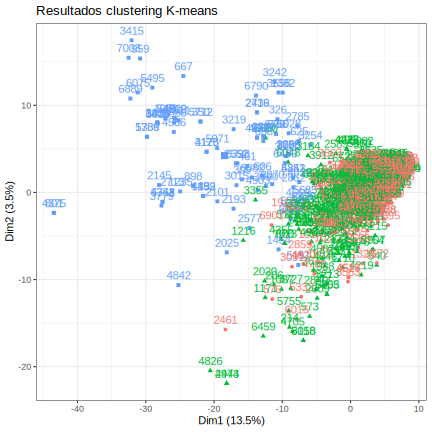
\includegraphics[width=\linewidth]{IMG/R2.png}
		\caption{K-means con distancia Euclidiana}
		\label{fig:r2}
	\end{subfigure}
	\caption{Comparación entre algoritmos con distancia Euclidiana}
\end{figure}



\begin{figure}[h!]
	\centering
	\begin{subfigure}[t]{0.45\textwidth}
		\centering
		\[
		\begin{bmatrix}
			5.0045 & 3.4155 & 1.4813 & 0.2533 \\
			5.8874 & 2.7578 & 4.3639 & 1.3990 \\
			6.7848 & 3.0544 & 5.6578 & 2.0553
		\end{bmatrix}
		\]
		\caption{Vectores de medias - Fuzzy C-means}
	\end{subfigure}
	\hspace{0.05\textwidth}
	\begin{subfigure}[t]{0.45\textwidth}
		\centering
		\[
		\begin{bmatrix}
			5.9016 & 2.7484 & 4.3935 & 1.4339 \\
			5.0060 & 3.4280 & 1.4620 & 0.2460 \\
			6.8500 & 3.0737 & 5.7421 & 2.0711
		\end{bmatrix}
		\]
		\caption{Vectores de medias - K-means}
	\end{subfigure}
	\caption{Comparación de los vectores de medias obtenidos por dos algoritmos}
\end{figure}

\newpage

El algoritmo convergió  en 18 iteraciones y a continuación se presentan las primeras 30 observaciones de la matriz de pertenencias del Fuzzy C-means.
\[
\begin{bmatrix}
	0.9984 & 0.0011 & 0.0005 \\
	0.9848 & 0.0108 & 0.0044 \\
	0.9877 & 0.0087 & 0.0037 \\
	0.9788 & 0.0150 & 0.0062 \\
	0.9972 & 0.0020 & 0.0009 \\
	0.9538 & 0.0325 & 0.0137 \\
	0.9874 & 0.0088 & 0.0037 \\
	0.9998 & 0.0001 & 0.0001 \\
	0.9501 & 0.0352 & 0.0147 \\
	0.9896 & 0.0074 & 0.0030 \\
	0.9795 & 0.0144 & 0.0062 \\
	0.9957 & 0.0031 & 0.0013 \\
	0.9811 & 0.0133 & 0.0055 \\
	0.9443 & 0.0385 & 0.0172 \\
	0.9166 & 0.0564 & 0.0270 \\
	0.8732 & 0.0856 & 0.0412 \\
	0.9637 & 0.0250 & 0.0113 \\
	0.9984 & 0.0011 & 0.0005 \\
	0.9286 & 0.0502 & 0.0212 \\
	0.9874 & 0.0088 & 0.0038 \\
	0.9797 & 0.0145 & 0.0057 \\
	0.9911 & 0.0062 & 0.0026 \\
	0.9726 & 0.0187 & 0.0087 \\
	0.9873 & 0.0092 & 0.0035 \\
	0.9784 & 0.0157 & 0.0060 \\
	0.9832 & 0.0121 & 0.0047 \\
	0.9973 & 0.0019 & 0.0008 \\
	0.9965 & 0.0025 & 0.0010 \\
	0.9967 & 0.0023 & 0.0010 \\
	0.9874 & 0.0090 & 0.0036
\end{bmatrix}
\]


\newpage

\subsection{Resultados para la distancia de Mahattan}

\begin{figure}[h!]
	\centering
	\begin{subfigure}[t]{0.48\textwidth}
		\centering
		\includegraphics[width=\linewidth]{IMG/R3.png}
		\caption{Fuzzy C-means con distancia Manhattan}
		\label{fig:r3}
	\end{subfigure}
	\hspace{0.02\textwidth}
	\begin{subfigure}[t]{0.48\textwidth}
		\centering
		\includegraphics[width=\linewidth]{IMG/R4.png}
		\caption{K-means con distancia Manhattan}
		\label{fig:r4}
	\end{subfigure}
	\caption{Comparación entre algoritmos con distancia Manhattan}
\end{figure}

\begin{figure}[h!]
	\centering
	\begin{subfigure}[t]{0.45\textwidth}
		\centering
		\[
		\begin{bmatrix}
			5.9295 & 2.7850 & 4.3955 & 1.4139 \\
			5.0104 & 3.4068 & 1.5099 & 0.2668 \\
			6.6007 & 3.0000 & 5.3743 & 1.9220
		\end{bmatrix}
		\]
		\caption{Vectores de medias - Fuzzy C-means}
	\end{subfigure}
	\hspace{0.05\textwidth}
	\begin{subfigure}[t]{0.45\textwidth}
		\centering
		\[
		\begin{bmatrix}
			5.9000 & 2.8000 & 4.5000 & 1.4000 \\
			5.0000 & 3.4000 & 1.5000 & 0.2000 \\
			6.7000 & 3.0000 & 5.7000 & 2.1000
		\end{bmatrix}
		\]
		\caption{Vectores de medias - K-means}
	\end{subfigure}
	\caption{Comparación de vectores de medias ajustados con la referencia}
\end{figure}

\newpage

El algoritmo convergió  en 18 iteraciones y a continuación se presentan las primeras 30 observaciones de la matriz de pertenencias del Fuzzy C-means.

\[
\begin{bmatrix}
	0.0019 & 0.9983 & 0.0010 \\
	0.0701 & 0.9980 & 0.0445 \\
	0.0159 & 0.9922 & 0.0083 \\
	0.0873 & 0.9967 & 0.0455 \\
	0.0051 & 0.9984 & 0.0035 \\
	0.0710 & 0.9810 & 0.0398 \\
	0.0264 & 0.9951 & 0.0119 \\
	0.0007 & 0.9999 & 0.0003 \\
	0.1409 & 0.9889 & 0.0687 \\
	0.0597 & 0.9989 & 0.0371 \\
	0.1168 & 0.9977 & 0.0551 \\
	0.0058 & 0.9978 & 0.0025 \\
	0.0567 & 0.9958 & 0.0322 \\
	0.0655 & 0.9658 & 0.0358 \\
	0.1977 & 0.9782 & 0.0998 \\
	0.2998 & 0.9759 & 0.1916 \\
	0.0609 & 0.9849 & 0.0351 \\
	0.0018 & 0.9985 & 0.0010 \\
	0.2190 & 0.9865 & 0.0931 \\
	0.0641 & 0.9985 & 0.0584 \\
	0.0393 & 0.9930 & 0.0141 \\
	0.0332 & 0.9985 & 0.0239 \\
	0.0232 & 0.9733 & 0.0128 \\
	0.0103 & 0.9923 & 0.0049 \\
	0.0155 & 0.9819 & 0.0070 \\
	0.1168 & 0.9989 & 0.0850 \\
	0.0023 & 0.9988 & 0.0011 \\
	0.0158 & 0.9994 & 0.0067 \\
	0.0053 & 0.9980 & 0.0022 \\
	0.0239 & 0.9956 & 0.0121 \\
	0.0349 & 0.9970 & 0.0195 
\end{bmatrix}
\]



\newpage

\section{Conclusiones}

Tras la realización de la aplicación, se pudo observar que entre el algoritmo Fuzzy y el K-means clásico, existen ligeras diferencias al momento de clasificar a un par de sujetos que se encuentran muy en la frontera de pertenecer a un grupo o a otro. Para este caso en particular, la distancia utilizada no tuvo un efecto tan relevante. 


\newpage

\section{Referencias}

\bibliographystyle{apalike}  % Estilo de cita, puedes cambiarlo si lo prefieres.
\bibliography{Biblio}         % Aquí incluyes el archivo .bib (sin extensión).

\newpage

\section{Anexos}

Este reporte se envía con los códigos anexos que corresponden a:

\begin{enumerate}
	\item El codigo en MATLAB del fuzzy cmeans  y kmeans con las pruebas

\end{enumerate}



\end{document}

